\documentclass[10pt,a4paper]{article}
\usepackage[margin=2cm]{geometry}
\usepackage[T1]{fontenc}
\usepackage{lmodern}
\usepackage{microtype}
\usepackage{amsmath,amssymb}
\usepackage{graphicx}
\usepackage{booktabs}
\usepackage{multirow}
\usepackage{subcaption}
\usepackage{caption}
\usepackage{enumitem}
\usepackage[dvipsnames]{xcolor}
\usepackage[colorlinks=true,linkcolor=MidnightBlue,citecolor=MidnightBlue,urlcolor=MidnightBlue]{hyperref}
\captionsetup{font=small,labelfont=bf}
\setlength{\parskip}{2pt}
% generated by experiments/make_figures.py -- do not edit
\newcommand{\nMainN}{24}
\newcommand{\nISNRMainTIKH}{5.41}
\newcommand{\nSSIMMainTIKH}{0.882}
\newcommand{\nWinsMainTIKH}{0}
\newcommand{\nWinsSSIMMainTIKH}{0}
\newcommand{\nISNRMainTV}{5.96}
\newcommand{\nSSIMMainTV}{0.891}
\newcommand{\nWinsMainTV}{1}
\newcommand{\nWinsSSIMMainTV}{1}
\newcommand{\nISNRMainTGV}{6.25}
\newcommand{\nSSIMMainTGV}{0.896}
\newcommand{\nWinsMainTGV}{10}
\newcommand{\nWinsSSIMMainTGV}{12}
\newcommand{\nISNRMainMULTI}{6.59}
\newcommand{\nSSIMMainMULTI}{0.897}
\newcommand{\nWinsMainMULTI}{13}
\newcommand{\nWinsSSIMMainMULTI}{11}
\newcommand{\nISNRMainAuto}{5.97}
\newcommand{\nSSIMMainAuto}{0.874}
\newcommand{\nISNRMainAutoS}{6.26}
\newcommand{\nSSIMMainAutoS}{0.894}
\newcommand{\nMainGainTGVGauss}{+0.73}
\newcommand{\nMainWinsGauss}{9}
\newcommand{\nMainNGauss}{12}
\newcommand{\nMainAutoGainTGVGauss}{+0.35}
\newcommand{\nMainGainTGVOof}{-0.06}
\newcommand{\nMainWinsOof}{4}
\newcommand{\nMainNOof}{12}
\newcommand{\nMainAutoGainTGVOof}{-0.91}
\newcommand{\nMainMultiBeatsTikh}{24}
\newcommand{\nMainMultiTikhGain}{1.18}
\newcommand{\nMainMultiBeatsTGV}{13}
\newcommand{\nMainAutoBeatsTGV}{10}
\newcommand{\nMainAutoBeatsTV}{12}
\newcommand{\nMainAutoBeatsTikh}{18}
\newcommand{\nMainAutoLoss}{0.62}
\newcommand{\nMainAutoLossMedian}{0.27}
\newcommand{\nMainAutoWithinHalf}{14}
\newcommand{\nMainAutoRelLoss}{7.8}
\newcommand{\nMainAutoRelLossMax}{32}
\newcommand{\nMainAutoSLoss}{0.33}
\newcommand{\nMainAutoSWithinHalf}{20}
\newcommand{\nMainAutoSRelLoss}{4.0}
\newcommand{\nMainAutoSRelLossMax}{22}
\newcommand{\nMainAutoSBeatsTGV}{13}
\newcommand{\nMainAutoSBeatsAuto}{16}
\newcommand{\nMainAutoSGainTGVGauss}{+0.56}
\newcommand{\nMainAutoSGainTGVOof}{-0.55}
\newcommand{\nTimeMainTIKH}{2.9}
\newcommand{\nTimeMainTV}{4.2}
\newcommand{\nTimeMainTGV}{27.3}
\newcommand{\nTimeMainMULTI}{16.1}
\newcommand{\nTimeMainAuto}{3.5}
\newcommand{\nTimeMainAutoS}{4.6}
\newcommand{\nKodakN}{24}
\newcommand{\nISNRKodakTIKH}{3.37}
\newcommand{\nSSIMKodakTIKH}{0.756}
\newcommand{\nWinsKodakTIKH}{0}
\newcommand{\nWinsSSIMKodakTIKH}{0}
\newcommand{\nISNRKodakTV}{4.26}
\newcommand{\nSSIMKodakTV}{0.812}
\newcommand{\nWinsKodakTV}{0}
\newcommand{\nWinsSSIMKodakTV}{3}
\newcommand{\nISNRKodakTGV}{4.31}
\newcommand{\nSSIMKodakTGV}{0.814}
\newcommand{\nWinsKodakTGV}{19}
\newcommand{\nWinsSSIMKodakTGV}{12}
\newcommand{\nISNRKodakMULTI}{3.92}
\newcommand{\nSSIMKodakMULTI}{0.803}
\newcommand{\nWinsKodakMULTI}{5}
\newcommand{\nWinsSSIMKodakMULTI}{9}
\newcommand{\nISNRKodakAuto}{3.77}
\newcommand{\nSSIMKodakAuto}{0.782}
\newcommand{\nISNRKodakAutoS}{3.75}
\newcommand{\nSSIMKodakAutoS}{0.789}
\newcommand{\nKodakGainTGVGauss}{-0.18}
\newcommand{\nKodakWinsGauss}{5}
\newcommand{\nKodakNGauss}{12}
\newcommand{\nKodakAutoGainTGVGauss}{-0.35}
\newcommand{\nKodakGainTGVOof}{-0.60}
\newcommand{\nKodakWinsOof}{0}
\newcommand{\nKodakNOof}{12}
\newcommand{\nKodakAutoGainTGVOof}{-0.73}
\newcommand{\nKodakMultiBeatsTikh}{22}
\newcommand{\nKodakMultiTikhGain}{0.55}
\newcommand{\nKodakMultiBeatsTGV}{5}
\newcommand{\nKodakAutoBeatsTGV}{4}
\newcommand{\nKodakAutoBeatsTV}{5}
\newcommand{\nKodakAutoBeatsTikh}{23}
\newcommand{\nKodakAutoLoss}{0.15}
\newcommand{\nKodakAutoLossMedian}{0.14}
\newcommand{\nKodakAutoWithinHalf}{21}
\newcommand{\nKodakAutoRelLoss}{1.8}
\newcommand{\nKodakAutoRelLossMax}{7}
\newcommand{\nKodakAutoSLoss}{0.18}
\newcommand{\nKodakAutoSWithinHalf}{22}
\newcommand{\nKodakAutoSRelLoss}{2.1}
\newcommand{\nKodakAutoSRelLossMax}{12}
\newcommand{\nKodakAutoSBeatsTGV}{3}
\newcommand{\nKodakAutoSBeatsAuto}{14}
\newcommand{\nKodakAutoSGainTGVGauss}{-0.32}
\newcommand{\nKodakAutoSGainTGVOof}{-0.81}
\newcommand{\nTimeKodakTIKH}{0.0}
\newcommand{\nTimeKodakTV}{0.3}
\newcommand{\nTimeKodakTGV}{4.8}
\newcommand{\nTimeKodakMULTI}{12.5}
\newcommand{\nTimeKodakAuto}{0.5}
\newcommand{\nTimeKodakAutoS}{0.5}
\newcommand{\nGainTGVSatellite}{-0.40}
\newcommand{\nGainTGVCthead}{+1.30}
\newcommand{\nGainTGVCat}{+0.28}
\newcommand{\nGainTGVPortrait}{+0.17}
\newcommand{\nRefined}{20}
\newcommand{\nEdgeTIKH}{1.065}
\newcommand{\nFlatTIKH}{1.335}
\newcommand{\nEdgeTV}{1.036}
\newcommand{\nFlatTV}{1.190}
\newcommand{\nEdgeTGV}{1.000}
\newcommand{\nFlatTGV}{1.000}
\newcommand{\nEdgeMULTI}{0.942}
\newcommand{\nFlatMULTI}{0.945}
\newcommand{\nEdgeAuto}{0.967}
\newcommand{\nFlatAuto}{1.066}
\newcommand{\nCollReMin}{0.0569}
\newcommand{\nCollReFinal}{0.1248}
\newcommand{\nCollKmin}{6}
\newcommand{\nCollKdisc}{3}
\newcommand{\nAutoDiscStops}{0}
\newcommand{\nKappa}{398}
\newcommand{\nKappaLoss}{9.1}
\newcommand{\nRatioLo}{2}
\newcommand{\nRatioHi}{380}
\newcommand{\nRatioSatLo}{2{,}179}
\newcommand{\nRatioSatHi}{51{,}449}
\newcommand{\nRfiveLoss}{0.7}
\newcommand{\nRfiveLossMax}{2.1}
\newcommand{\nRoneLoss}{8.8}
\newcommand{\nRoneLossMax}{29}
\newcommand{\nRfifteenLoss}{4.7}
\newcommand{\nRfifteenLossMax}{12}
\newcommand{\nColParrotsTGVPSNR}{29.12}
\newcommand{\nColParrotsTGVSSIM}{0.868}
\newcommand{\nColParrotsAutoPSNR}{28.22}
\newcommand{\nColParrotsAutoSSIM}{0.806}
\newcommand{\nColParrotsBlurPSNR}{23.84}
\newcommand{\nColParrotsBlurSSIM}{0.758}
\newcommand{\nColBikesTGVPSNR}{24.45}
\newcommand{\nColBikesTGVSSIM}{0.777}
\newcommand{\nColBikesAutoPSNR}{23.92}
\newcommand{\nColBikesAutoSSIM}{0.760}
\newcommand{\nColBikesBlurPSNR}{18.47}
\newcommand{\nColBikesBlurSSIM}{0.313}
\newcommand{\nScaleBest}{0.5}
\newcommand{\nLoioSigMean}{14.7}
\newcommand{\nLoioSigMedian}{2.4}
\newcommand{\nLoioSigMax}{133}
\newcommand{\nLoioSigCat}{9.7}
\newcommand{\nLoioSigCthead}{8.1}
\newcommand{\nLoioSigPortrait}{8.4}
\newcommand{\nLoioSigSatellite}{32.6}
\newcommand{\nLoioBestMean}{5.0}
\newcommand{\nLoioBestMedian}{1.4}
\newcommand{\nLoioBestMax}{33}
\newcommand{\nLoioBestCat}{0.7}
\newcommand{\nLoioBestCthead}{3.5}
\newcommand{\nLoioBestPortrait}{0.9}
\newcommand{\nLoioBestSatellite}{14.9}
\newcommand{\nScaleC}{7.5}
\newcommand{\nKRLoN}{24}
\newcommand{\nKRLoAuto}{4.83}
\newcommand{\nKRLoAutoS}{4.74}
\newcommand{\nKRLoGain}{-0.09}
\newcommand{\nKRLoWins}{11}
\newcommand{\nKRLoBestGain}{0.25}
\newcommand{\nKRLoWorstGain}{-0.92}
\newcommand{\nKRLoRelRE}{+1.1}
\newcommand{\nKRHiN}{24}
\newcommand{\nKRHiAuto}{1.77}
\newcommand{\nKRHiAutoS}{2.48}
\newcommand{\nKRHiGain}{+0.71}
\newcommand{\nKRHiWins}{22}
\newcommand{\nKRHiBestGain}{2.64}
\newcommand{\nKRHiWorstGain}{-0.04}
\newcommand{\nKRHiRelRE}{-7.5}
\newcommand{\nStopMinLoss}{5.1}
\newcommand{\nFloorMinLoss}{+0.3}
\newcommand{\nFloorBetter}{17}
\newcommand{\nWorstPlain}{2.04}
\newcommand{\nWorstStop}{1.35}
\newcommand{\nWorstFloor}{1.72}
\newcommand{\nVarNoneMean}{5.70}
\newcommand{\nVarNoneWorst}{-1.61}
\newcommand{\nVarNoneLoss}{0.89}
\newcommand{\nVarNoneWithin}{16}
\newcommand{\nVarStopMean}{4.74}
\newcommand{\nVarStopWorst}{-2.85}
\newcommand{\nVarStopLoss}{1.85}
\newcommand{\nVarStopWithin}{6}
\newcommand{\nVarFloorMean}{5.97}
\newcommand{\nVarFloorWorst}{0.07}
\newcommand{\nVarFloorLoss}{0.62}
\newcommand{\nVarFloorWithin}{14}
\newcommand{\nVarScaleMean}{6.26}
\newcommand{\nVarScaleWorst}{1.86}
\newcommand{\nVarScaleLoss}{0.33}
\newcommand{\nVarScaleWithin}{20}

\input{missing}
% a figure/table that has not been generated yet shows up as a red box
\let\oldincludegraphics\includegraphics
\renewcommand{\includegraphics}[2][]{\IfFileExists{#2}{\oldincludegraphics[#1]{#2}}{\fbox{\textcolor{red}{missing: \detokenize{#2}}}}}
\newcommand{\inputtable}[1]{\IfFileExists{#1}{\input{#1}}{\fbox{\textcolor{red}{missing: \detokenize{#1}}}}}

\title{\textbf{Automatic Pixel-Wise Multi-Penalty Regularization\\for Image Deblurring and Denoising}\\[4pt]
\large CS663 Digital Image Processing --- Course Project}
\author{Kushagra Kushwaha (24b2191) \and Siddhesh Sangram Phadke (24b4502)}
\date{November 2026}

\begin{document}
\maketitle

\begin{abstract}
\noindent
We re-implement from scratch, in Python, the MULTI method of Bortolotti, Landi
and Zama~\cite{multi}. MULTI restores a blurred, noisy image by giving
\emph{every pixel its own} Tikhonov regularisation weight and choosing all $N$
weights automatically through a ``uniform penalty'' fixed-point rule. The model
is solved by an outer fixed-point loop on the weights, and the inner problem is
solved by a Newton Projection method whose Hessian is approximated by an
FFT-diagonalisable (BCCB) matrix. We reproduce the paper's protocol (Gaussian and
out-of-focus blur, three noise levels, four image types) and compare against
Tikhonov, Total Variation and Total Generalised Variation solvers that we also
wrote ourselves. Beyond reproduction, we
(i) measure edge-region versus flat-region errors and line profiles to explain
\emph{where} MULTI wins;
(ii) map MULTI's sensitivity to $\epsilon$ and to the neighbourhood size $R$;
(iii) find and explain a failure mode we call \emph{$\lambda$-collapse}, a
positive feedback loop between the residual and the weights that makes the
fixed-point iteration semi-convergent, and fix it by flooring the rule's noise
estimate at a robust (MAD) noise level, which removes the catastrophic failures at no cost;
(iv) build a fully automatic, ground-truth-free variant (MULTI-auto), improve it with an
$\epsilon$ that follows the image's curvature scale (MULTI-autoS), and test both on unseen
Kodak images; and
(v) extend MULTI to colour images.
\end{abstract}

\section{Introduction}
\label{sec:intro}

Out-of-focus optics, atmospheric turbulence and motion all blur images, and every
sensor adds noise. Recovering the sharp image is an ill-posed inverse problem.
Inverse filtering divides by the blur's frequency response, which is close to
zero at high frequencies, so the noise explodes (as seen in the Fourier and
denoising parts of the course). Variational methods stabilise the inversion by
adding a regularisation term weighted by a parameter $\lambda$. Two
difficulties remain:
\begin{enumerate}[leftmargin=*,itemsep=1pt]
\item \textbf{Choosing $\lambda$.} Too small amplifies noise, too large
  over-smooths. In practice $\lambda$ is tuned by hand, or by looking at
  the ground truth, which is not available in real use.
\item \textbf{One $\lambda$ for the whole image.} Flat regions would benefit from
  strong smoothing and edges from almost none. A single global weight has to
  compromise between the two. Edge-preserving regularisers such as TV and TGV
  work around this with non-quadratic penalties, but they still have one
  global $\lambda$, and they bring their own artefacts (staircasing for TV).
\end{enumerate}

MULTI~\cite{multi} tackles both at once. It keeps the simplest, quadratic
Laplacian penalty but uses $N$ weights $\lambda_i$, one per pixel. All of them
are set automatically by a closed-form rule, derived from the \emph{uniform
penalty} principle~\cite{upen}, which makes $\lambda_i$ inversely proportional
to the local curvature of the restored image. Only one scalar, $\epsilon$,
remains to be chosen.

\paragraph{Objectives (as approved).}
\begin{itemize}[leftmargin=*,itemsep=1pt]
\item Implement MULTI (Algorithm~1 of the paper) together with its Newton Projection
  inner solver, using a BCCB/FFT Hessian approximation.
\item Test it on Gaussian and out-of-focus (radius~5) blur at noise levels
  $0.5\%$, $1\%$ and $2.5\%$, and compare against Tikhonov, TV and TGV using RE,
  ISNR and SSIM, with a visual study of edges and smooth regions.
\item If time permits: sensitivity to the neighbourhood size and to $\epsilon$;
  colour images; generalisation to other datasets (Kodak).
\end{itemize}
All objectives were completed, and the optional ones are covered in
Secs.~\ref{sec:ablation}--\ref{sec:color}.

\paragraph{Our contributions beyond reproduction.}
Following the instructor's advice to be creative in evaluation and insight:
\begin{itemize}[leftmargin=*,itemsep=1pt]
\item An \emph{edge vs.\ flat} error decomposition, line profiles and $\lambda$-maps,
  which show \emph{where} pixel-wise adaptivity helps and where it does not.
\item A dense $\epsilon$-sweep, which shows that the best $\epsilon$ is set mainly by
  the \emph{image content}, not by the noise level.
\item The discovery and analysis of \emph{$\lambda$-collapse}, a semi-convergence of
  Algorithm~1 that the paper does not discuss, and a one-line fix (a noise floor
  in the $\lambda$ rule, in the spirit of the discrepancy principle~\cite{morozov})
  that removes the catastrophic failures without hurting the good cases.
\item MULTI-auto: a variant with no hand-tuned parameter and no ground truth, and
  MULTI-autoS, which sets $\epsilon$ from the curvature scale of a cheap pilot restoration;
  both are evaluated on held-out Kodak images. Plus a channel-wise colour extension.
\end{itemize}

\section{Background}
\label{sec:background}

\paragraph{Degradation model.}
A blurred and noisy observation $\mathbf b\in\mathbb R^N$ of an unknown image
$\mathbf u\in\mathbb R^N$ (both vectorised, $N=n_x n_y$) is modelled as
\begin{equation}
  A\mathbf u + \mathbf e = \mathbf b ,
  \label{eq:model}
\end{equation}
where $A$ is the convolution with the point spread function (PSF) and $\mathbf e$
is white Gaussian noise. We use the noise level $\delta=\|\mathbf e\|/\|A\mathbf u\|$,
as in the paper. Inverting $A$ directly (inverse filtering) amplifies noise at the
frequencies where $|\hat A|$ is small. The problem is ill-posed, so it must be
\emph{regularised}:
\begin{equation}
  \min_{\mathbf u\ge 0}\ \tfrac12\|A\mathbf u-\mathbf b\|^2 + \mathcal R(\mathbf u).
  \label{eq:variational}
\end{equation}

\paragraph{Periodic boundaries, BCCB matrices and the FFT.}
With periodic boundary conditions, every convolution (the blur $A$, the discrete
Laplacian $L$ and the finite-difference gradient $D$) is a block-circulant
matrix with circulant blocks (BCCB). The 2-D DFT diagonalises all of them
simultaneously (the convolution theorem from the Fourier-transform lectures):
$A=F^{*}\operatorname{diag}(\hat a)F$, $L=F^{*}\operatorname{diag}(\hat\ell)F$, with
$\hat a=\mathrm{fft2}(\text{PSF})$ and
$\hat\ell_{pq}=2\cos(2\pi p/n_x)+2\cos(2\pi q/n_y)-4$.
Any matrix of the form $A^TA+\mu L^TL$ is therefore inverted in $O(N\log N)$ by
\[
(A^TA+\mu L^TL)^{-1}\mathbf g
  = F^{*}\!\left[\frac{F\mathbf g}{|\hat a|^2+\mu\,\hat\ell^{\,2}}\right].
\]
We use this fact both in MULTI's inner solver and in all of the baselines.

\paragraph{Classical single-parameter regularisers.}
\begin{itemize}[leftmargin=*,itemsep=1pt]
\item \textbf{Tikhonov (TIKH):} $\mathcal R=\frac{\lambda}{2}\|L\mathbf u\|^2$.
  It is quadratic and fast, but it penalises edges as much as noise, so it
  over-smooths edges.
\item \textbf{Total variation (TV)}~\cite{rof}: $\mathcal R=\lambda\sum_i\|(D\mathbf u)_i\|_2$.
  It preserves edges, but it favours piecewise-constant solutions, which shows up as
  \emph{staircasing} in smooth ramps.
\item \textbf{Total generalised variation (TGV$^2$)}~\cite{tgv}:
  $\mathcal R=\min_{\mathbf v}\ \alpha_1\|D\mathbf u-\mathbf v\|_{1}+\alpha_0\|\mathcal E\mathbf v\|_{1}$,
  where $\mathcal E$ is the symmetrised gradient. It favours piecewise-\emph{affine}
  images, which removes the staircasing of TV. It is the strongest baseline in the paper.
\end{itemize}
Each of these methods has a single global $\lambda$. It has to be hand-tuned, and
the same amount of smoothing is applied to flat regions, textures and edges.

\section{The MULTI method}
\label{sec:multi}

\subsection{Model}
MULTI~\cite{multi} uses one regularisation parameter \emph{per pixel}
($p=N$ penalties in the multi-penalty framework
$\mathcal R=\sum_i\lambda_i\psi_i$) and sets them automatically:
\begin{equation}
\begin{aligned}
\mathbf u^{*} &= \arg\min_{\mathbf u\ge 0}\ \tfrac12\|A\mathbf u-\mathbf b\|^2
     + \tfrac12\sum_{i=1}^{N}\lambda_i^{*}(L\mathbf u)_i^2, \\
\lambda_i^{*} &= \frac{\|A\mathbf u^{*}-\mathbf b\|^2}{N\big(S_i+\epsilon\big)},
\qquad S_i=\max_{j\in\mathcal N_i}(L\mathbf u^{*})_j^2 ,
\end{aligned}
\label{eq:multi}
\end{equation}
where $\mathcal N_i$ is the $R\times R$ window centred on pixel $i$ and
$\epsilon>0$ is a small threshold.

\paragraph{Intuition: the uniform penalty principle.}
Wherever $S_i\gg\epsilon$, equation~\eqref{eq:multi} gives
$\lambda_i (L\mathbf u)_i^2\approx\|A\mathbf u-\mathbf b\|^2/N$. Every pixel then
pays roughly the \emph{same} penalty, equal to the mean squared residual (that is,
the noise variance $\sigma^2$ at the discrepancy level). The weight
$\lambda_i$ is therefore \emph{inversely proportional to the local curvature}:
\begin{itemize}[leftmargin=*,itemsep=1pt]
\item at edges and fine structures $|L\mathbf u|$ is large, so $\lambda_i$ is small
  and the detail is preserved;
\item in flat regions $|L\mathbf u|\approx 0$, so $\lambda_i\to\|A\mathbf u-\mathbf b\|^2/(N\epsilon)$,
  which is large, and noise is smoothed strongly.
\end{itemize}
The $R\times R$ max filter widens the low-$\lambda$ zone around an edge, since the
Laplacian of an edge is a thin double ridge that passes through zero exactly at the
edge. The constant $\epsilon$ caps the largest $\lambda$ and decides which
curvatures count as ``flat''. Note that MULTI with a constant $\lambda$ \emph{is}
TIKH with the same Laplacian penalty. Our TIKH baseline therefore isolates exactly
what the pixel-wise adaptivity contributes.

\subsection{Algorithm 1: fixed-point iteration on $\boldsymbol\lambda$}
Starting from $\mathbf u^{(0)}=\mathbf b$, with
$\boldsymbol\lambda^{(0)}$ given by~\eqref{eq:multi}, repeat:

\begin{center}
\fbox{\begin{minipage}{0.92\linewidth}
\begin{enumerate}[leftmargin=*,itemsep=1pt,label=\arabic*:]
\item $\mathbf u^{(k+1)}=\arg\min_{\mathbf u\ge0}\ \frac12\|A\mathbf u-\mathbf b\|^2+\frac12\sum_i\lambda_i^{(k)}(L\mathbf u)_i^2$
      \hfill (Newton Projection, warm start $\mathbf u^{(k)}$)
\item $S_i^{(k+1)}=\max_{j\in\mathcal N_i}(L\mathbf u^{(k+1)})_j^2$ \hfill (max filter, periodic)
\item $\lambda_i^{(k+1)}=\|A\mathbf u^{(k+1)}-\mathbf b\|^2/\big(N(S_i^{(k+1)}+\epsilon)\big)$
\item stop when $\|\boldsymbol\lambda^{(k+1)}-\boldsymbol\lambda^{(k)}\|\le\mathrm{Tol}\,\|\boldsymbol\lambda^{(k+1)}\|$ \hfill ($\mathrm{Tol}=10^{-1}$, at most 20 iterations)
\end{enumerate}
\end{minipage}}
\end{center}

\subsection{Inner solver: modified Newton Projection (NP)}
For a fixed $\boldsymbol\lambda$, the objective
$\mathcal J(\mathbf u)=\frac12\|A\mathbf u-\mathbf b\|^2+\frac12\sum_i\lambda_i(L\mathbf u)_i^2$
is a strictly convex quadratic with gradient
$\mathbf g=A^T(A\mathbf u-\mathbf b)+L^T\Lambda L\mathbf u$ and Hessian
$A^TA+L^T\Lambda L$. The Hessian is \emph{not} BCCB, because $\Lambda$ varies
spatially. Following the paper, we replace it with the BCCB approximation
\begin{equation}
  H = A^TA+\mu L^TL,\qquad \mu=\operatorname{mean}(\lambda_1,\dots,\lambda_N),
  \label{eq:H}
\end{equation}
which is inverted with two FFTs. One NP iteration is:
\begin{enumerate}[leftmargin=*,itemsep=1pt]
\item Compute the active set
  $\mathcal I=\{i:\ 0\le u_i\le\varepsilon_k,\ g_i>0\}$, with
  $\varepsilon_k=\min\{\bar\varepsilon,\ \|\mathbf u-[\mathbf u-\mathbf g]^+\|\}$.
  These are the pixels pinned at the bound $u\ge0$.
\item Compute the reduced gradient $\mathbf g_{\mathcal I}$ ($=\mathbf g$ with the
  entries in $\mathcal I$ set to zero), solve $H\mathbf d=\mathbf g_{\mathcal I}$ by FFT,
  and set $p_i=d_i$ for $i\notin\mathcal I$ and $p_i=g_i$ for $i\in\mathcal I$.
\item Projected Armijo search: take $\alpha=\beta^m$ ($\beta=0.5$, $\eta=10^{-4}$), the first value for which
  $\mathcal J(\mathbf u)-\mathcal J([\mathbf u-\alpha\mathbf p]^+)\ \ge\ \eta\big(\alpha\sum_{i\notin\mathcal I}g_ip_i+\sum_{i\in\mathcal I}g_i(u_i-[\mathbf u-\alpha\mathbf p]^+_i)\big)$,
  and set $\mathbf u\leftarrow[\mathbf u-\alpha\mathbf p]^+$.
\end{enumerate}
The NP iterations stop when the relative change in $\mathbf u$ or the relative
projected-gradient norm falls below $10^{-5}$, or after 1000 iterations. Because $H$ is
constant and positive definite, the convergence theory of~\cite{landi2012} applies.
One NP iteration costs about 6 FFTs of size $N$.

\paragraph{Implementation notes (our code).}
Everything is written from scratch in Python/NumPy (\texttt{src/}): operators and
FFT eigenvalues (\texttt{operators.py}), MULTI and NP (\texttt{multi.py}), and the
baselines (\texttt{baselines.py}). We added one safeguard that the paper does not
mention. If $\sum_{i\notin\mathcal I}g_ip_i\le0$, which can happen because $H^{-1}$ couples
free and active pixels, we fall back to the projected-gradient direction.
In our runs this safeguard almost never triggers.

\section{Experimental setup}
\label{sec:setup}

\paragraph{Test images.}
The paper's images (\texttt{galaxy}, \texttt{mri}, \texttt{leopard}, \texttt{elaine})
are not freely redistributable; the paper itself notes that they are standard
images rather than a published dataset. We therefore replaced each one with a
freely available image \emph{of the same kind}, so that every image category the
paper tests is still represented (Fig.~\ref{fig:testimages}):
\begin{itemize}[leftmargin=*,itemsep=1pt]
\item \textbf{satellite} ($256^2$, RestoreTools~\cite{hno}) stands in for
  \texttt{galaxy}: an astronomical image with a black background and thin,
  bright structures. Like the paper's galaxy, it uses $R=3$.
\item \textbf{ct\_head} ($256^2$, a scikit-image CT slice) stands in for
  \texttt{mri}: a medical image with large homogeneous regions and sharp
  anatomical boundaries.
\item \textbf{cat} ($256^2$, scikit-image \texttt{chelsea}) stands in for
  \texttt{leopard}: fur texture, whiskers and eyes.
\item \textbf{portrait} ($512^2$, Kodak \texttt{kodim04}) stands in for
  \texttt{elaine}: a woman in a hat, with smooth skin and sharp contours.
\end{itemize}
For the generalisation study (Sec.~\ref{sec:kodak}), we use 12 further Kodak
images~\cite{kodak}, converted to grayscale and resized to $256^2$
(Fig.~\ref{fig:kodak}), with both blurs at $\delta=10^{-2}$ (24 more problems; we
kept to one noise level to limit the computational cost). All intensities lie in $[0,1]$.

\begin{figure}[t]
\centering
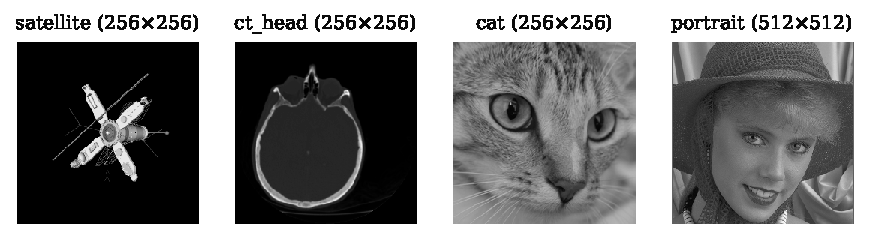
\includegraphics[width=\linewidth]{figures/test_images.pdf}\\[2pt]
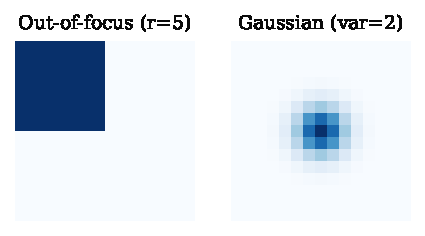
\includegraphics[width=0.48\linewidth]{figures/psfs.pdf}
\caption{Top: the four main test images. Bottom: the two PSFs (central $15\times15$ crop).}
\label{fig:testimages}
\end{figure}

\paragraph{Degradations.}
These follow the paper exactly: (i) a Gaussian PSF with variance 2 (the equivalent
of RestoreTools' \texttt{psfGauss}), and (ii) an out-of-focus disk of radius 5 (the
equivalent of MATLAB's \texttt{fspecial('disk',5)}; boundary pixels are weighted by
their area inside the disk). Both use periodic convolution. Gaussian noise is added
at levels $\delta\in\{2.5\times10^{-2},\,10^{-2},\,5\times10^{-3}\}$, which gives
$4\times2\times3=24$ test problems. The noise seed is fixed per problem, so every
method sees the same $\mathbf b$.

\paragraph{Metrics.}
These are the paper's metrics: relative error
$\mathrm{RE}=\|\hat{\mathbf u}-\mathbf u\|/\|\mathbf u\|$,
$\mathrm{ISNR}=20\log_{10}(\|\mathbf b-\mathbf u\|/\|\hat{\mathbf u}-\mathbf u\|)$ (dB),
and the mean SSIM~\cite{ssim} (Gaussian window, $\sigma=1.5$). We also report PSNR.

\paragraph{Baselines and solvers.}
All methods include the constraint $\mathbf u\ge0$ and use periodic boundaries.
The paper used MATLAB codes (SGP, ADMM, RESPOND), which we do not have, so we
implemented equivalent solvers ourselves:
\begin{itemize}[leftmargin=*,itemsep=1pt]
\item \textbf{TIKH} ($\frac\lambda2\|L\mathbf u\|^2$): solved with the same NP solver.
  Here $H$ is the \emph{exact} Hessian, so NP converges in a few iterations.
\item \textbf{TV}: ADMM~\cite{admm} with splittings $\mathbf z=D\mathbf u$ and $\mathbf w=\mathbf u$; the
  $\mathbf u$-step is an FFT solve, the $\mathbf z$-step an isotropic shrinkage, and the
  $\mathbf w$-step a projection. At most 400 iterations.
\item \textbf{TGV$^2$} ($\alpha_1=\lambda$, $\alpha_0=2\lambda$): the primal--dual hybrid
  gradient method of Chambolle and Pock~\cite{cp}, with the data term dualised so that every
  proximal map is closed-form. We tuned the primal/dual step ratio (30) by checking
  that the objective plateaus; it reaches the minimiser in about 1500 iterations
  (limit 2000).
\end{itemize}

\paragraph{Parameter selection.}
As in the paper, the single parameter of each baseline ($\lambda$ for TIKH, TV
and TGV) and $\epsilon$ for MULTI are chosen to \emph{minimise RE} against the
ground truth. This is an \emph{oracle}, best-case choice for every method. We
implemented it as a coarse log-grid search followed by golden-section refinement,
which expands the bracket automatically if the optimum lies on its edge
(\texttt{experiments/common.py}). MULTI's $\epsilon$ is tuned with a cap of
2000 total NP iterations per run. The reported MULTI run then uses the paper's
full budget (20 outer iterations $\times$ 1000 NP iterations) at the tuned $\epsilon$.
The dense $\epsilon$-sweep of Sec.~\ref{sec:ablation} showed that RE$(\epsilon)$ is not
always unimodal, so a local golden-section search can miss the global optimum. For
every problem we therefore also refine around the best point of the 21-value sweep,
and we keep whichever of the two results is better. This makes the ``oracle'' MULTI
genuinely best-case, like the baselines.
\textbf{MULTI-auto} (Sec.~\ref{sec:auto}) uses no ground truth at all.

\paragraph{MULTI settings.}
These are the paper's values: $\mathrm{Tol}=10^{-1}$ with at most 20 outer
iterations; NP tolerance $10^{-5}$ with at most 1000 iterations;
$R=5$ ($R=3$ for satellite).

\section{Results: reproducing the paper's comparison}
\label{sec:results}

\subsection{Quantitative comparison}
Table~\ref{tab:summary} averages the four metrics over the 24 problems.
The full per-problem tables, in the paper's format (RE, ISNR, MSSIM, iterations and
the chosen parameter), are in Appendix~\ref{app:tables}.

\begin{table}[t]
\centering\small
\inputtable{tables/summary.tex}
\caption{Mean metrics over all problems. ``best ISNR/MSSIM'' counts the problems on
which a method is best among all six rows. MULTI-autoS is MULTI-auto with the
scale-aware $\epsilon$ of Sec.~\ref{sec:auto}; the Kodak rows are discussed in
Sec.~\ref{sec:kodak}. Times are medians in seconds, single-threaded,
for the final run only (parameter tuning is not included). MULTI-auto runs once with no
tuning, so its time is its entire cost, whereas the tuned methods need 10--20 runs each
to choose their parameter.}
\label{tab:summary}
\end{table}

\paragraph{MULTI vs.\ TIKH: what pixel-wise adaptivity buys.}
TIKH is exactly MULTI with a single, constant $\lambda$ (same penalty, same solver).
The difference between the two therefore isolates the effect of the
$N$ pixel-wise weights. MULTI beats TIKH on \nMainMultiBeatsTikh/\nMainN{} problems,
by \nMainMultiTikhGain\,dB ISNR on average. The gap is largest where the image
combines large flat areas with sharp structures (satellite and ct\_head under
out-of-focus blur, up to $+5$\,dB). There TIKH must choose between leaving noise
in the background and blurring the edges, whereas MULTI does not have to choose.

\paragraph{MULTI vs.\ TGV/TV: it depends on the blur.}
The comparison with the edge-preserving regularisers splits cleanly along the PSF.
\begin{itemize}[leftmargin=*,itemsep=1pt]
\item \textbf{Gaussian blur}: MULTI is the best of the four tuned methods on
  \nMainWinsGauss/\nMainNGauss{} problems, \nMainGainTGVGauss\,dB above TGV on average.
\item \textbf{Out-of-focus blur}: TGV wins on most problems, and MULTI is on
  average \nMainGainTGVOof\,dB behind it (MULTI is best on \nMainWinsOof/\nMainNOof).
\end{itemize}
This is the same pattern as in the paper's Tables~2--5, where MULTI dominates under
Gaussian blur while TGV wins several out-of-focus cases (for example
\texttt{elaine}). Per image, the mean ISNR gap MULTI$-$TGV is
\nGainTGVCthead\,dB (ct\_head), \nGainTGVCat\,dB (cat), \nGainTGVPortrait\,dB (portrait)
and \nGainTGVSatellite\,dB (satellite).
Our explanation is as follows. The out-of-focus PSF has a disk-shaped support,
so its spectrum has \emph{zeros} (rings at the zeros of the Bessel function $J_1$).
Information at those frequencies is lost and has to be \emph{filled in} by the
prior. A sparsity prior on the gradient (TV) or on the second derivative (TGV)
fills in sharp edges, which is exactly what a disk blur has destroyed. A quadratic
penalty, however locally weighted, fills them in with smooth, ringing-prone
content. The Gaussian PSF has no spectral zeros, only a smooth decay, so
nothing has to be filled in, and MULTI's smaller bias (a quadratic penalty does not shrink
contrast the way an $\ell_1$ penalty does) wins.

\paragraph{The satellite image.}
Satellite is the hardest case for MULTI. 90\% of its pixels are exactly zero (black
background), and the best $\epsilon$ is huge ($\sim\!10^{-1}$, see Sec.~\ref{sec:ablation}).
With such an $\epsilon$, MULTI behaves like TIKH in most of the image (a constant
$\lambda$), with reduced $\lambda$ only on the bright structures. TV/TGV are
better here because a piecewise-constant prior is nearly exact for this image.
The non-negativity constraint is active on a large fraction of the pixels, which
also makes the Newton Projection solver slow on this image (many backtracking steps).

\subsection{Visual study: edges and smooth regions}
Figures~\ref{fig:rest-oof}--\ref{fig:zooms} show the restorations. Two artefacts
are clearly visible. TIKH leaves grainy noise in flat regions and halos around edges.
TV makes smooth shading on the face and in the background look like flat
``cartoon'' patches. TGV and MULTI both avoid TV's staircasing. At normal viewing scale, the differences among
TV, TGV and MULTI are subtle (all are within about 1\,dB). The most visible ones are TV's
blotchy patches on the cat's fur and the portrait's forehead, and the slightly finer fur and hair
texture that MULTI keeps. The edge/flat decomposition below makes these
differences measurable.

\begin{figure}[p]
\centering
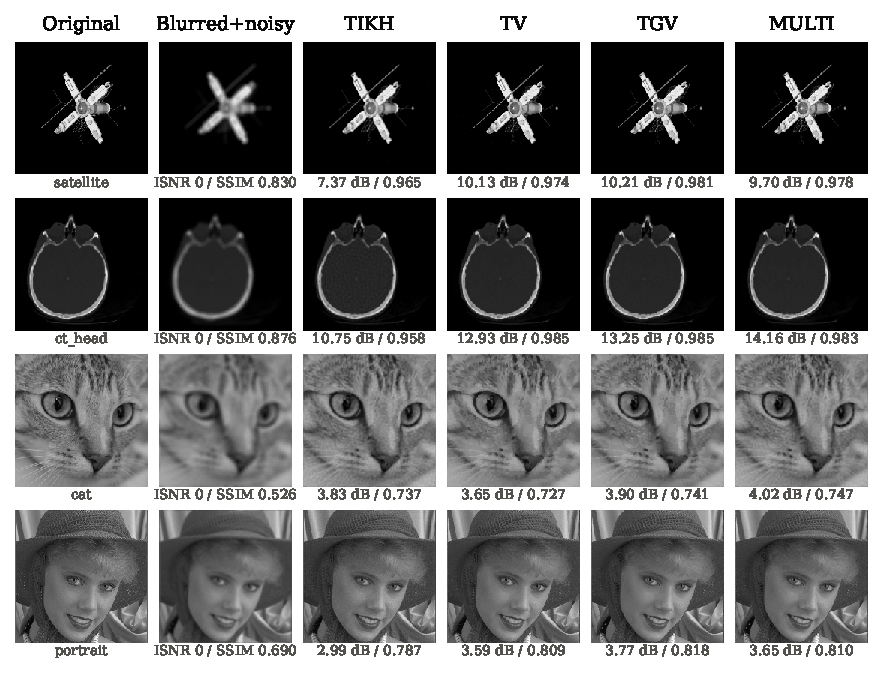
\includegraphics[width=\linewidth]{figures/restorations_oof.pdf}
\caption{Out-of-focus blur, $\delta=10^{-2}$. Below each image: ISNR (dB) / MSSIM.}
\label{fig:rest-oof}
\vspace{6pt}
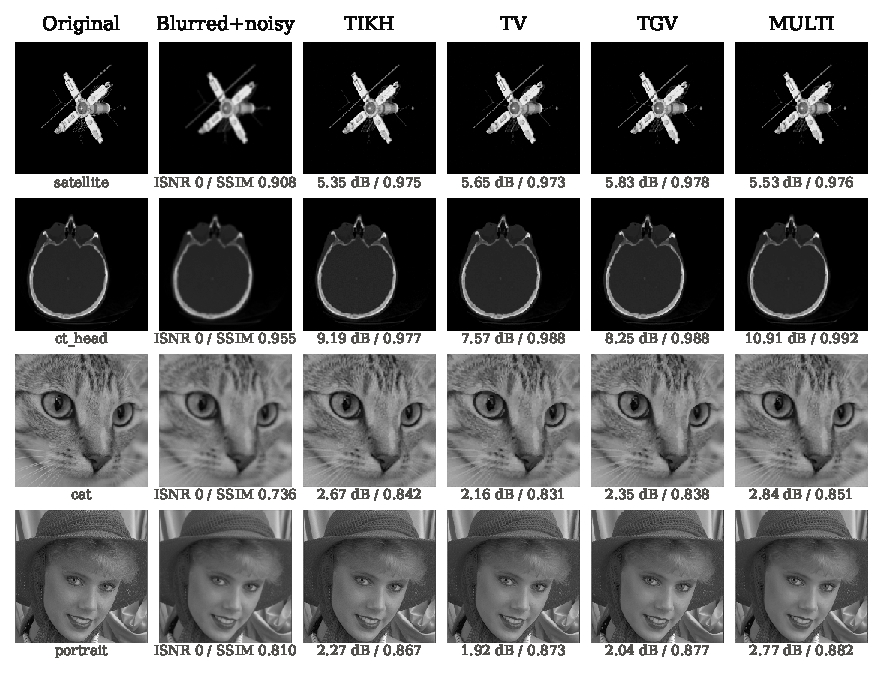
\includegraphics[width=\linewidth]{figures/restorations_gauss.pdf}
\caption{Gaussian blur, $\delta=10^{-2}$.}
\label{fig:rest-gauss}
\end{figure}

\begin{figure}[t]
\centering
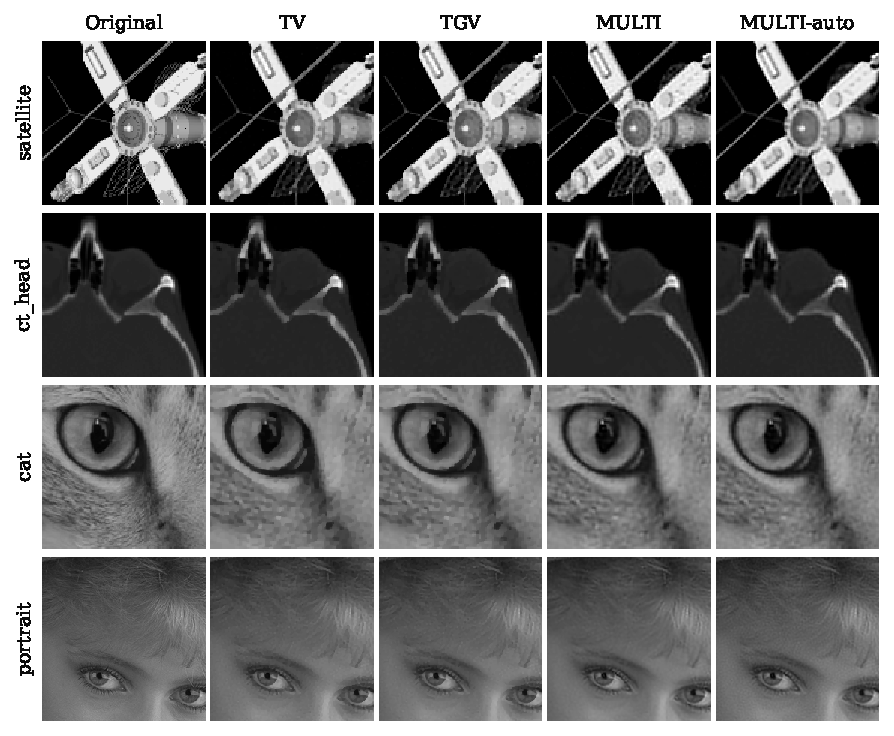
\includegraphics[width=0.9\linewidth]{figures/zooms_gauss.pdf}
\caption{Zoomed crops (Gaussian blur, $\delta=10^{-2}$). Note TV's patchy fur and forehead
texture, and the finer texture retained by MULTI.}
\label{fig:zooms}
\end{figure}

\paragraph{Edge vs.\ flat error decomposition.}
To quantify ``edges and smooth regions'', we split the pixels of every ground truth
using the smoothed gradient magnitude: the top 15\% are \emph{edge} pixels and the
bottom 50\% are \emph{flat} pixels. We then compute the RMSE of each method on each
class separately, relative to TGV (geometric mean over the 24 problems,
Fig.~\ref{fig:regions}). The result is instructive:
\begin{itemize}[leftmargin=*,itemsep=1pt]
\item TIKH and TV lose mostly in \emph{flat} regions, by
  $\times$\nFlatTIKH{} and $\times$\nFlatTV{}: noise in TIKH, and staircase patches in TV.
\item MULTI matches TGV in flat regions ($\times$\nFlatMULTI) and is
  \emph{better at edges} ($\times$\nEdgeMULTI). Its advantage comes from detail
  preservation, because low $\lambda_i$ is placed exactly where the curvature is large.
\item MULTI-auto keeps part of MULTI's edge advantage ($\times$\nEdgeAuto) but loses in
  flat regions ($\times$\nFlatAuto). At high noise its automatic $\epsilon$ is too large, so
  $\boldsymbol\lambda$ is too small and noise survives in flat areas (Sec.~\ref{sec:auto}).
\end{itemize}

\begin{figure}[t]
\centering
\begin{minipage}[t]{0.47\linewidth}\vspace{0pt}
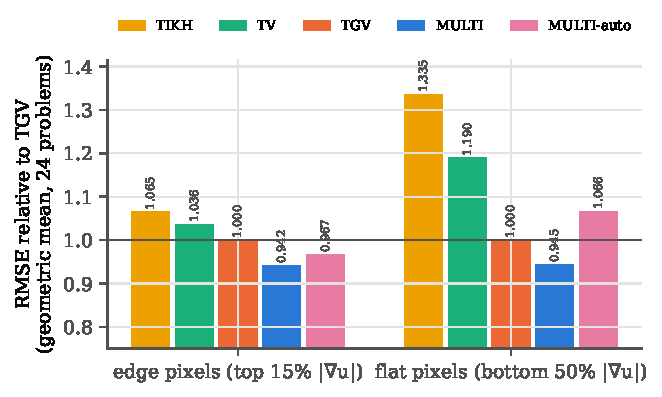
\includegraphics[width=\linewidth]{figures/region_rmse.pdf}
\caption{RMSE on edge and flat pixels relative to TGV (below 1 is better).}
\label{fig:regions}
\end{minipage}\hfill
\begin{minipage}[t]{0.5\linewidth}\vspace{0pt}
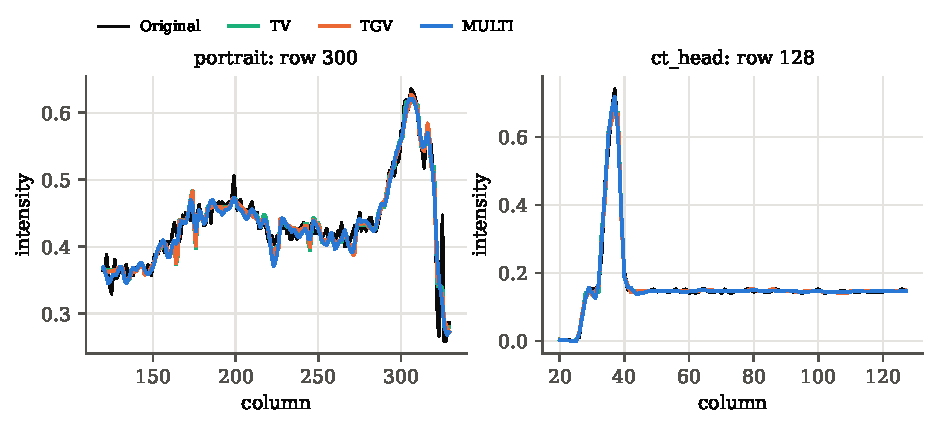
\includegraphics[width=\linewidth]{figures/profiles_oof.pdf}\\
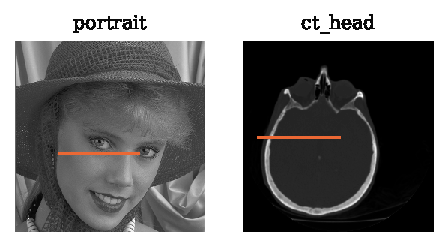
\includegraphics[width=0.75\linewidth]{figures/profiles_location.pdf}
\caption{Line profiles (out-of-focus, $\delta=10^{-2}$) and their locations.}
\label{fig:profiles}
\end{minipage}
\end{figure}

\paragraph{What the $\lambda$ map looks like.}
Figure~\ref{fig:lambda} shows the final $\boldsymbol\lambda$ of MULTI on a log scale.
It acts as an \emph{edge detector}: $\lambda_i$ is several orders of magnitude
smaller on the outlines (skull, fur pattern, hat, satellite arms) than in flat areas.
The ``thick'' outlines come from the $R\times R$ max filter, which merges the two lobes of
the Laplacian's zero crossing. In effect, MULTI performs edge detection (the course's
Laplacian/zero-crossing material) and edge-aware denoising together, inside one
variational problem.

\begin{figure}[t]
\centering
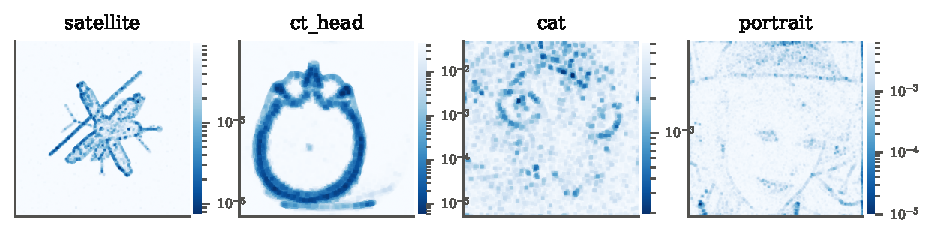
\includegraphics[width=\linewidth]{figures/lambda_maps_oof.pdf}
\caption{Final regularisation-parameter maps $\lambda_i$ of MULTI (log colour scale,
out-of-focus, $\delta=10^{-2}$). Dark means small $\lambda$, i.e.\ little smoothing.}
\label{fig:lambda}
\end{figure}

\begin{figure}[t]
\centering
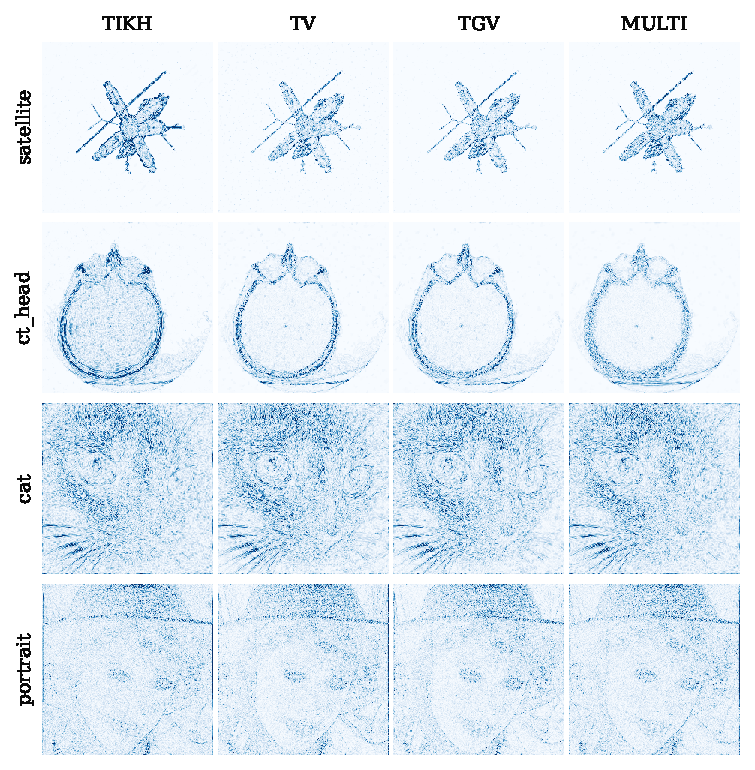
\includegraphics[width=0.8\linewidth]{figures/errormaps_oof.pdf}
\caption{Absolute error maps (out-of-focus, $\delta=10^{-2}$, common colour scale per
row). TIKH's error is spread over the flat regions; the errors of all the other methods concentrate on edges.}
\label{fig:errmaps}
\end{figure}

\section{Sensitivity and convergence of MULTI}
\label{sec:ablation}

\subsection{The threshold $\epsilon$}
We ran MULTI for 21 log-spaced values $\epsilon\in[10^{-5},10^{-1}]$ on all 24 problems
(Fig.~\ref{fig:eps}).
\begin{itemize}[leftmargin=*,itemsep=1pt]
\item \textbf{Flat optimum, steep cliff.} RE$(\epsilon)$ is nearly flat over
  1--2 decades below the optimum and then rises steeply. Choosing $\epsilon$
  too \emph{small} is cheap: $\lambda$ becomes unbounded in flat regions, but the
  data term and the curvature term still balance. Choosing it too \emph{large}
  is expensive: $\lambda_i\approx\|A\mathbf u-\mathbf b\|^2/(N\epsilon)$ becomes small and
  uniform, so noise is under-regularised everywhere.
\item \textbf{The best $\epsilon$ is set by the image, not by the noise.} Within one
  image the oracle $\epsilon$ hardly changes with $\delta$ (right panel; points of one
  colour lie on a near-horizontal band). Across images it spans three
  decades: about $10^{-4}$ for ct\_head, about $3\times10^{-3}$ for cat/portrait and
  about $6\times10^{-2}$ for satellite. As a result, the ratio $\epsilon_{\rm opt}/\hat\sigma^2$
  ranges from \nRatioLo{} to \nRatioHi{} for the natural and medical images, and from
  \nRatioSatLo{} to \nRatioSatHi{} for satellite.
  This contradicts the natural guess $\epsilon\propto\sigma^2$, which we had used
  for our first automatic rule. The explanation is that $\epsilon$ is compared with $S_i$,
  the \emph{restored} curvature, which reflects the image content much more
  than the noise.
\end{itemize}

\begin{figure}[t]
\centering
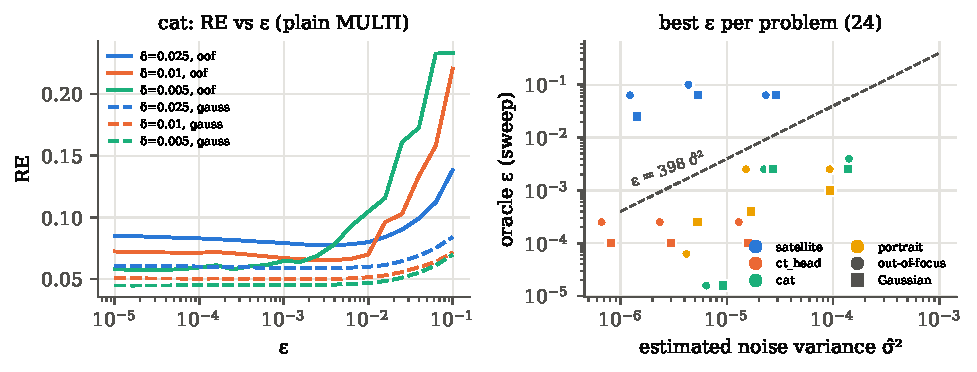
\includegraphics[width=0.85\linewidth]{figures/eps_sweep.pdf}
\caption{Left: RE vs.\ $\epsilon$ for cat (solid: out-of-focus, dashed: Gaussian).
Right: the best $\epsilon$ of every problem against the estimated noise variance.
The best $\epsilon$ clusters by image, not along the line $\epsilon\propto\hat\sigma^2$.}
\label{fig:eps}
\end{figure}

\subsection{The neighbourhood size $R$}
For every $R\in\{1,3,5,9,15\}$ we re-tuned $\epsilon$ ($\delta=10^{-2}$, both blurs,
Fig.~\ref{fig:R}). The best $R$ is 3 or 5 for every problem. $R=1$, i.e.\ no max filter,
is clearly worse (on average $+\nRoneLoss\%$ RE relative to the best $R$, up to
$+\nRoneLossMax\%$ on ct\_head). The Laplacian of an edge changes sign
exactly at the edge, so without the max filter $\lambda_i$ is \emph{large} on the edge
itself and the edge gets smoothed. Large windows hurt too, though less
($R=15$: $+\nRfifteenLoss\%$ on average, up to $+\nRfifteenLossMax\%$): the low-$\lambda$ zone
around every edge widens, so noise survives next to edges. The paper's default $R=5$ is on
average within \nRfiveLoss\% of the best $R$ (at worst \nRfiveLossMax\%). Satellite prefers
$R=3$, which agrees with the paper's choice of $R=3$ for its galaxy image; ct\_head, with its
thin bone and soft-tissue contours, is the most sensitive to $R$ in both directions.

\begin{figure}[t]
\centering
\begin{minipage}[t]{0.49\linewidth}\vspace{0pt}
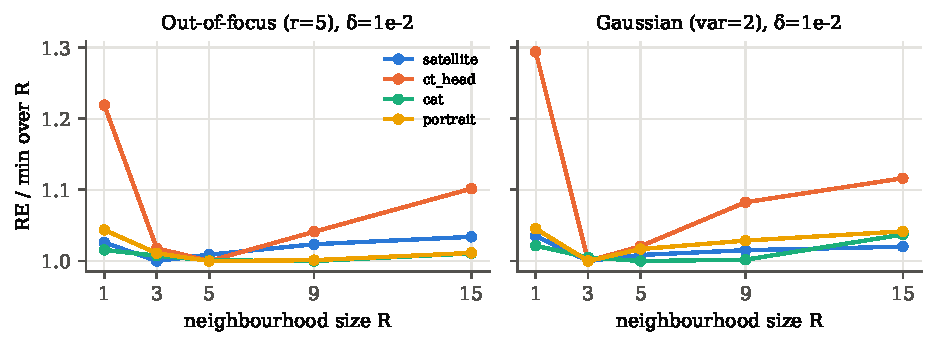
\includegraphics[width=\linewidth]{figures/R_sweep.pdf}
\caption{RE (relative to the best $R$) vs.\ neighbourhood size; $\epsilon$ re-tuned for each $R$.}
\label{fig:R}
\end{minipage}\hfill
\begin{minipage}[t]{0.49\linewidth}\vspace{0pt}
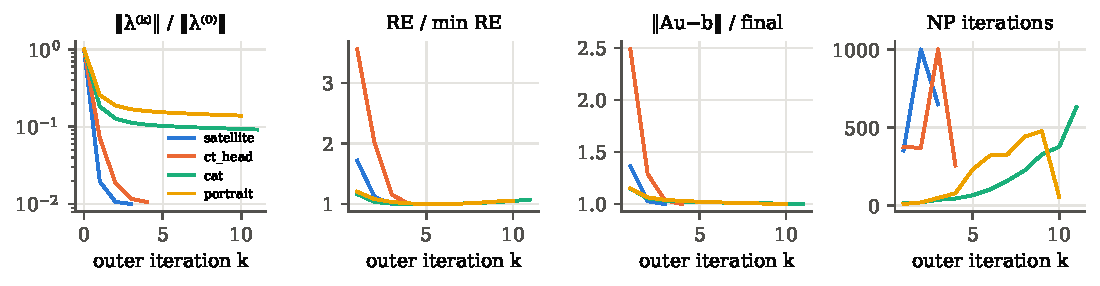
\includegraphics[width=\linewidth]{figures/convergence.pdf}
\caption{Algorithm~1 histories (out-of-focus, $\delta=10^{-2}$, oracle $\epsilon$, $\mathrm{Tol}=0$).}
\label{fig:conv}
\end{minipage}
\end{figure}

\subsection{Convergence of Algorithm~1}
With $\mathrm{Tol}=0$ (Fig.~\ref{fig:conv}), as in the paper's Figure~10, $\|\boldsymbol\lambda\|$
drops by one to two orders of magnitude in the first 2--4 outer iterations and then
settles. RE reaches its minimum after 3--5 outer iterations, and the residual
stabilises at the same time. The cost of an outer iteration grows as $\boldsymbol\lambda$
becomes more heterogeneous, because the BCCB preconditioner, built from the
\emph{mean} $\lambda$, then fits the true Hessian less well, so NP needs more iterations. The
paper's $\mathrm{Tol}=10^{-1}$ stops after 3--5 outer iterations, close to the RE
minimum. Note, however, that RE starts to \emph{rise} again for cat and portrait. This
leads to the failure mode in the next section.

\section{Extension 1: $\lambda$-collapse and a noise-floor safeguard}
\label{sec:collapse}
Our first automatic variant (Sec.~\ref{sec:auto}) failed catastrophically on two
problems, cat and portrait under out-of-focus blur at $\delta=0.5\%$, where it gave
\emph{negative} ISNR ($-1.6$\,dB, worse than the blurred input). The iteration
histories (Fig.~\ref{fig:collapse}) reveal a positive feedback loop in
Algorithm~1:
\begin{center}
residual $\|A\mathbf u-\mathbf b\|$ below the noise level
$\Rightarrow$ $\lambda_i\propto\|A\mathbf u-\mathbf b\|^2$ shrinks
$\Rightarrow$ the next solve fits more noise
$\Rightarrow$ the residual drops further $\Rightarrow\dots$
\end{center}
The numerator of $\lambda_i$ is the current residual, which is an estimate of the noise
energy $N\sigma^2$. Once the solution starts to over-fit, this estimate becomes
\emph{biased low}, and nothing in the rule pulls it back up. $\|\boldsymbol\lambda\|$ then
decays geometrically, so the $\lambda$-change test ($\mathrm{Tol}$) never fires
and the iteration runs for all 20 outer iterations. On cat, RE falls to
\nCollReMin{} at outer iteration \nCollKmin{} and then climbs back to \nCollReFinal.
This is the classical \emph{semi-convergence} of iterative regularisation~\cite{engl},
appearing here in a fixed-point method that is supposed to be ``automatic''.
It occurs when $\epsilon$ is large relative to the curvature scale and the noise is low.
In the paper's oracle setting, a too-large $\epsilon$ is simply never selected, which is
probably why the paper does not report it.

\paragraph{Fix, first attempt: discrepancy stop.} The residual should never fall
below the noise level. Our first fix stops Algorithm~1 as soon as
$\|A\mathbf u^{(k)}-\mathbf b\|\le\tau\sqrt N\,\hat\sigma$ ($\tau=1$), which is Morozov's
discrepancy principle~\cite{morozov}. Here $\hat\sigma$ is the robust MAD noise estimate
from the finest diagonal Haar wavelet coefficients,
$\hat\sigma=\mathrm{median}|HH|/0.6745$~\cite{donoho}, so no ground truth is needed.
This removes the catastrophic failures (stars in Fig.~\ref{fig:collapse}), but the dense
$\epsilon$-sweep shows that it stops \emph{too early}: usually after 1--2 outer
iterations, before $\boldsymbol\lambda$ has adapted to the image. Its best RE is on average
\nStopMinLoss\% worse than that of the plain algorithm.

\paragraph{Fix, final: a noise floor in the $\lambda$ rule.} The root cause is that
the numerator of $\lambda_i$ can drop below the true noise energy. We therefore floor it:
\begin{equation}
\lambda_i=\frac{\max\big(\|A\mathbf u-\mathbf b\|^2,\ N\hat\sigma^2\big)}{N\,(S_i+\epsilon)} .
\label{eq:floor}
\end{equation}
While the residual is above the noise level, this is exactly the paper's rule. When the
residual would fall below it, the overall scale of $\boldsymbol\lambda$ is frozen at the
discrepancy level, but the iteration continues to refine \emph{where} the smoothing goes
(through $S_i$). The positive feedback loop is broken, and the usual $\mathrm{Tol}$ test
then terminates the iteration. The cost is one scalar $\max$ per outer iteration.
Over the sweep (Fig.~\ref{fig:epssafe}), the floored algorithm's best RE differs from that of
the plain algorithm by \nFloorMinLoss\% on average (equal or better on \nFloorBetter/24
problems), so nothing is lost when no collapse occurs. It is also less sensitive to
$\epsilon$: the median ratio of worst to best RE over the four decades of $\epsilon$ drops
from \nWorstPlain{} (plain) to \nWorstFloor{}. This sweep caps every run at 2000 NP
iterations, which cuts the collapse short and therefore \emph{understates} the benefit.
With the full budget used by MULTI-auto (Table~\ref{tab:variants}), the floor raises the
worst-case ISNR from \nVarNoneWorst\,dB (no safeguard) and \nVarStopWorst\,dB (discrepancy
stop) to \nVarFloorWorst\,dB, and gives the best mean ISNR (\nVarFloorMean\,dB) and the
smallest average loss to the oracle (\nVarFloorLoss\,dB). The plain rule is within
0.5\,dB of the oracle slightly more often (\nVarNoneWithin{} vs.\ \nVarFloorWithin{} of 24),
but it fails badly on the problems where it collapses.

\begin{table}[t]
\centering\small
\inputtable{tables/auto_variants.tex}
\caption{MULTI-auto on the 24 main problems with each $\lambda$-collapse safeguard
($\kappa$ re-calibrated for each variant on its own $\epsilon$-sweep, except ``none'', which
uses our initial calibration). ISNR and MSSIM are means; ``worst'' is the worst single
problem; ``loss'' is the mean ISNR gap to oracle-tuned MULTI, and the last column counts the
problems within 0.5\,dB of it. The last row is MULTI-autoS (Sec.~\ref{sec:auto}).}
\label{tab:variants}
\end{table}

\begin{figure}[t]
\centering
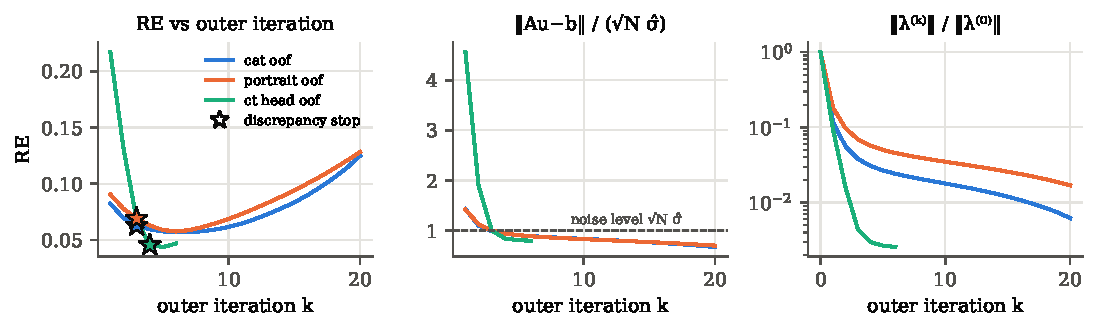
\includegraphics[width=\linewidth]{figures/lambda_collapse.pdf}
\caption{$\lambda$-collapse of MULTI with automatic $\epsilon$ and no safeguard
(out-of-focus, $\delta=0.5\%$). Once the residual crosses the noise level (dashed),
$\|\boldsymbol\lambda\|$ keeps decaying and RE grows. Stars: where the discrepancy
stop (our first fix) would end the iteration.}
\label{fig:collapse}
\end{figure}

\section{Extension 2: fully automatic MULTI (MULTI-auto)}
\label{sec:auto}
The paper chooses $\epsilon$ by minimising RE against the ground truth, which is not
possible in real use. MULTI-auto sets
\[
\epsilon=\kappa\,\hat\sigma^2,\qquad \text{with the noise-floor rule~\eqref{eq:floor}},
\]
with one global constant $\kappa$, calibrated once on the 24 main problems and then
\emph{frozen}. The calibration minimises the mean relative RE loss with respect to the
per-problem oracle $\epsilon$, read off the noise-floor sweep (Fig.~\ref{fig:epssafe}, right);
it gives $\kappa=\nKappa$. The rationale is dimensional: $\epsilon$ is a curvature
threshold, and the variance of the discrete Laplacian of pure noise is $20\sigma^2$.
Note that this rule is at odds with our sweep, where the best $\epsilon$ barely grows with
$\sigma$ (Sec.~\ref{sec:ablation}); we return to this below.

\paragraph{Results on the main set.} With no tuning at all, MULTI-auto is on average
\nMainAutoLoss\,dB (median \nMainAutoLossMedian\,dB) below oracle-tuned MULTI,
and within 0.5\,dB of it on \nMainAutoWithinHalf/\nMainN{} problems. It beats
oracle-tuned TIKH on \nMainAutoBeatsTikh, oracle TV on \nMainAutoBeatsTV{} and oracle
TGV on \nMainAutoBeatsTGV{} of the \nMainN{} problems. Each oracle baseline needed
10--20 runs \emph{and the ground truth} to choose its parameter. In RE terms the average
loss is \nMainAutoRelLoss\%, but the worst problem loses \nMainAutoRelLossMax\%. The large
losses are all at $\delta=2.5\%$, where $\kappa\hat\sigma^2$ overshoots the best
$\epsilon$ by about an order of magnitude. Since $\lambda_i\propto 1/(S_i+\epsilon)$, the weights
then become roughly $15\times$ too small and almost uniform: MULTI under-regularises, leaves
noise in flat regions and loses most of its adaptivity.

\begin{figure}[t]
\centering
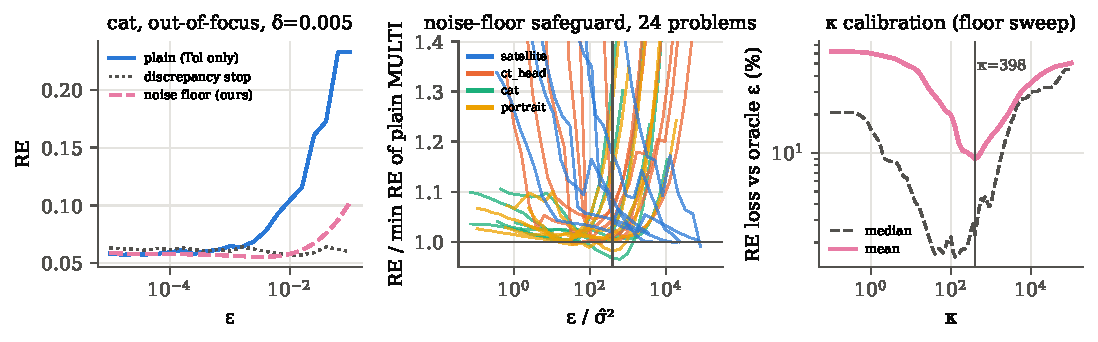
\includegraphics[width=\linewidth]{figures/eps_safe.pdf}
\caption{Left: RE vs.\ $\epsilon$ on the collapse case for plain MULTI and both safeguards.
Middle: noise-floor RE$(\epsilon)$ for all 24 problems, relative to the best RE of plain MULTI.
Right: calibration of $\kappa$ (mean and median relative RE loss over the 24 problems).}
\label{fig:epssafe}
\end{figure}

\paragraph{A scale-aware alternative.} Since the best $\epsilon$ follows the image's
curvature scale (Sec.~\ref{sec:ablation}), we also tried
$\epsilon=c\cdot Q_q\big(S(\mathbf u_{\rm pilot})\big)$, a quantile of the local curvature
of a cheap pilot restoration. The pilot is Laplacian-Tikhonov with $\lambda$ set by the
discrepancy principle, solved in closed form by FFT, which costs about 40 FFT solves.
We evaluated it against the $\kappa\hat\sigma^2$ rule with \emph{leave-one-image-out}
calibration: the constant is fitted on three images and tested on the
fourth. With $\epsilon$ read off the sweep curves, the best quantile ($q=\nScaleBest$, $c\approx\nScaleC$
when fitted on all four images) gives a mean held-out RE loss of \nLoioBestMean\% with respect
to the per-problem oracle $\epsilon$ (median \nLoioBestMedian\%, worst \nLoioBestMax\%). The
$\kappa\hat\sigma^2$ rule, evaluated the same way, gives \nLoioSigMean\% (median
\nLoioSigMedian\%, worst \nLoioSigMax\%). Per held-out image, the scale-aware rule loses
\nLoioBestCat\% (cat), \nLoioBestPortrait\% (portrait), \nLoioBestCthead\% (ct\_head) and
\nLoioBestSatellite\% (satellite), against \nLoioSigCat\%, \nLoioSigPortrait\%,
\nLoioSigCthead\% and \nLoioSigSatellite\% for $\kappa\hat\sigma^2$. Satellite is the hardest
case for both rules: its best $\epsilon$ lies at the upper end of the sweep grid, and at small
$\epsilon$ many of its sweep runs hit the NP budget, so its curves are the least reliable.

\paragraph{Full runs: MULTI-autoS.} The sweep curves are only a proxy (2000-NP cap), so we also
ran the rule for real. MULTI-autoS uses $\epsilon=c\,Q_{\nScaleBest}(S(\mathbf u_{\rm pilot}))$
with $c=\nScaleC$, the noise floor and the full budget; nothing else changes. On the main set
(where $c$ is in-sample) it is on average \nMainAutoSLoss\,dB below oracle MULTI, against
\nMainAutoLoss\,dB for MULTI-auto; it is within 0.5\,dB of the oracle on
\nMainAutoSWithinHalf/\nMainN{} problems (MULTI-auto: \nMainAutoWithinHalf), and its worst RE
loss drops from \nMainAutoRelLossMax\% to \nMainAutoSRelLossMax\%
(Table~\ref{tab:variants}, last row). The gain is concentrated at $\delta=2.5\%$, exactly where
$\kappa\hat\sigma^2$ overshoots.

For a held-out test we ran both automatic rules on the 12 Kodak images at the two noise levels
where they differ (no oracle needed). At $\delta=2.5\%$, MULTI-autoS is better on
\nKRHiWins/\nKRHiN{} problems, by \nKRHiGain\,dB ISNR on average (up to \nKRHiBestGain\,dB;
mean RE change \nKRHiRelRE\%). At $\delta=0.5\%$ the two rules are level
(\nKRLoGain\,dB on average, better on \nKRLoWins/\nKRLoN{}, worst \nKRLoWorstGain\,dB), and at
$\delta=1\%$, where $\kappa$ is effectively calibrated, they are also level
(\nISNRKodakAutoS{} vs.\ \nISNRKodakAuto\,dB, Table~\ref{tab:kodak}). So the scale-aware rule
removes the high-noise failure of $\kappa\hat\sigma^2$ with no systematic loss elsewhere, at the cost of
one pilot solve (about 40 FFTs). We keep $\kappa\hat\sigma^2$ as ``MULTI-auto'' in the main
tables because it was fixed before these experiments; MULTI-autoS is reported alongside it.



\section{Extension 3: generalisation to unseen Kodak images}
\label{sec:kodak}
To check that the conclusions are not specific to four hand-picked images, we
repeated the comparison on 12 Kodak images that were not used for any design
decision (Fig.~\ref{fig:kodak}). There are \nKodakN{} problems: both blurs at $\delta=1\%$.
TIKH, TV, TGV and MULTI are again oracle-tuned per problem, while MULTI-auto uses the
\emph{frozen} $\kappa=\nKappa$.

\begin{figure}[t]
\centering
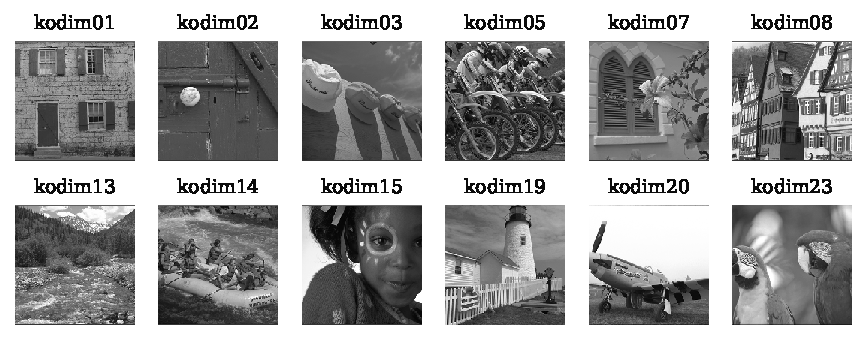
\includegraphics[width=0.9\linewidth]{figures/kodak_images.pdf}
\caption{The 12 Kodak generalisation images (grayscale, $256^2$).}
\label{fig:kodak}
\end{figure}

\begin{figure}[t]
\centering
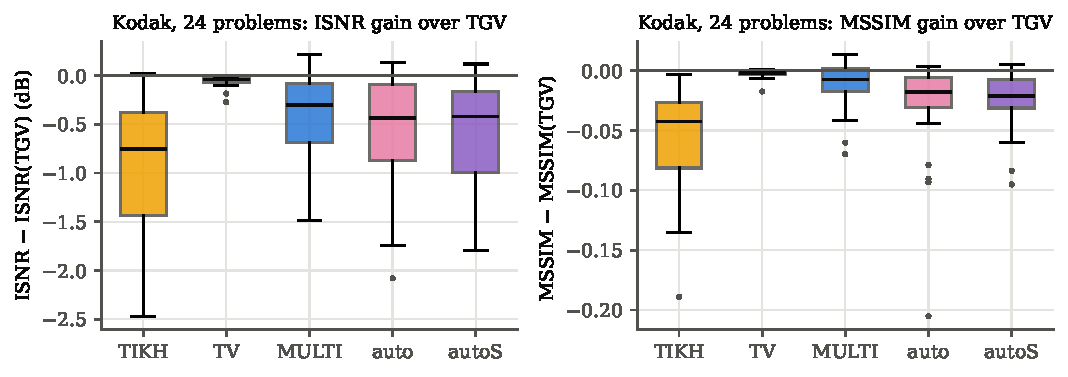
\includegraphics[width=0.9\linewidth]{figures/kodak_gain.pdf}
\caption{Kodak: per-problem ISNR and MSSIM difference with respect to oracle TGV.}
\label{fig:kodakgain}
\end{figure}

\begin{table}[t]
\centering\small
\inputtable{tables/kodak_isnr.tex}
\caption{Kodak: mean ISNR (dB) per blur.}
\label{tab:kodak}
\end{table}

The blur dependence carries over, but in a milder form (Fig.~\ref{fig:kodakgain},
Table~\ref{tab:kodak}). Under Gaussian blur, MULTI and TGV are close: MULTI is on average
\nKodakGainTGVGauss\,dB from TGV and is the best tuned method on \nKodakWinsGauss/\nKodakNGauss{}
images. Under out-of-focus blur TGV is clearly ahead (\nKodakGainTGVOof\,dB; MULTI best on
\nKodakWinsOof/\nKodakNOof). So MULTI's Gaussian-blur advantage on the main set does not
generalise to these small, texture-rich photographs, where TGV's sparsity prior pays off.
MULTI still beats TIKH, which uses the same penalty, on \nKodakMultiBeatsTikh/\nKodakN{}
problems (by \nKodakMultiTikhGain\,dB on average). MULTI-auto, which never saw these images, is
on average only \nKodakAutoLoss\,dB below oracle MULTI and within 0.5\,dB of it on
\nKodakAutoWithinHalf/\nKodakN{} problems.

\section{Extension 4: colour images}
\label{sec:color}
MULTI extends to RGB with no change to the model: we run MULTI-auto independently on
each channel, each with its own $\hat\sigma$, $\epsilon$ and $\boldsymbol\lambda$ map. As a baseline,
we run channel-wise TGV with a single $\lambda$ that is oracle-tuned on the colour RE.
On \texttt{kodim23} (parrots) and \texttt{kodim05} (motorbikes) with out-of-focus blur
at $\delta=1\%$ (Fig.~\ref{fig:color}), MULTI-auto reaches
\nColParrotsAutoPSNR\,dB / SSIM \nColParrotsAutoSSIM{} and
\nColBikesAutoPSNR\,dB / \nColBikesAutoSSIM{}, against
\nColParrotsTGVPSNR\,dB / \nColParrotsTGVSSIM{} and \nColBikesTGVPSNR\,dB / \nColBikesTGVSSIM{}
for oracle TGV (blurred input: \nColParrotsBlurPSNR{} and \nColBikesBlurPSNR\,dB).
Without any tuning, MULTI-auto gains 4.4--5.5\,dB over the blurred input and stays within
1\,dB of ground-truth-tuned TGV, in line with the grayscale out-of-focus results. Its SSIM
deficit on the parrots comes from the smooth, defocused background: the three channels get
independent $\boldsymbol\lambda$ maps, so noise that survives in one channel but not in the
others appears as coloured speckle, which the eye (and SSIM) notices more than grey noise.
A natural improvement is a single curvature map $S_i$, computed from the luminance (or as
$\max_c S_i^{(c)}$) and shared by all channels.

\begin{figure}[t]
\centering
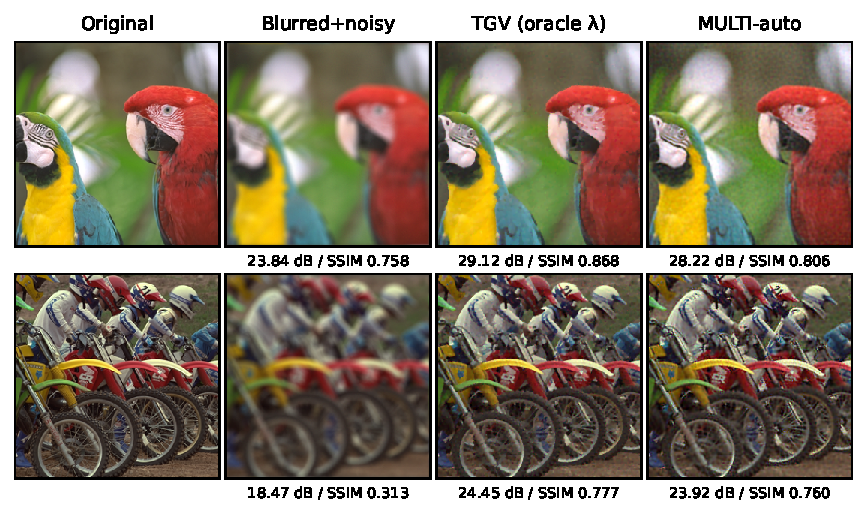
\includegraphics[width=0.9\linewidth]{figures/color.pdf}
\caption{Colour restoration (out-of-focus, $\delta=1\%$), channel-wise. Below each image: PSNR / SSIM.}
\label{fig:color}
\end{figure}

\section{Insights and limitations}
\label{sec:insights}

\begin{enumerate}[leftmargin=*,itemsep=2pt]
\item \textbf{A quadratic penalty with the right weights is competitive with
  non-smooth regularisers.} MULTI uses the oldest penalty there is,
  $\|L\mathbf u\|^2$, yet it matches or beats TGV whenever the blur has no spectral
  zeros. The weights do the edge-preserving job that the $\ell_1$ norm does in TV/TGV,
  and they avoid TV's contrast loss and staircasing. Each subproblem stays a smooth
  quadratic, so it can be solved with a Newton-type method and FFTs.

\item \textbf{The prior matters most where the blur destroys information.} Under
  out-of-focus blur, whose PSF has spectral zeros, the sparsity prior of TGV fills in
  the lost frequencies better. This is a limit of the quadratic model, not of the
  solver, and it suggests that applying pixel-wise weights to a TGV penalty could
  combine the strengths of both.

\item \textbf{``Automatic'' fixed-point rules can be semi-convergent.} The
  uniform-penalty update uses the current residual as its noise estimate. If the
  solution over-fits, the estimate is biased low and the error feeds back on itself
  ($\lambda$-collapse). Flooring that estimate at an external (MAD) noise level fixes
  this at negligible cost, and works better than simply stopping at the discrepancy level,
  which halts the adaptation too early. We consider this the most practically
  important finding of the project.

\item \textbf{$\epsilon$ is an image-scale parameter, not a noise parameter.}
  The best $\epsilon$ varies by three decades between images but hardly with the
  noise level. A single constant times $\hat\sigma^2$ works only because the
  RE$(\epsilon)$ curve is flat on its small-$\epsilon$ side, especially with the
  safeguard. Setting $\epsilon$ from the curvature scale of a cheap pilot restoration
  (MULTI-autoS) fixes the rule's failures at high noise: on held-out Kodak images at
  $\delta=2.5\%$ it gains \nKRHiGain\,dB over $\kappa\hat\sigma^2$.

\item \textbf{Cost.} One MULTI run costs about as much as TGV (tens of seconds in our
  single-threaded Python). Its cost is dominated by NP iterations, which increase when
  $\boldsymbol\lambda$ is very heterogeneous (the mean-$\lambda$ BCCB preconditioner then
  fits poorly) and when many pixels sit on the bound $u=0$ (satellite).
  A better preconditioner, for example a few CG steps on the true Hessian, could
  reduce this cost.
\end{enumerate}

\paragraph{Limitations of our study.}
(i) We used freely available stand-ins for the paper's four test images, so our
numbers are not directly comparable with the paper's tables; the qualitative
pattern is what we reproduce.
(ii) Our TV/TGV solvers are our own ADMM/PDHG codes rather than the paper's MATLAB packages.
We checked their convergence (TGV with 3$\times$ more iterations changes RE only in the 4th digit).
(iii) The oracle comparison is best-case for every method and does not reflect how
$\lambda$ would be chosen in practice. Only MULTI-auto is a fair real-world method.
(iv) To limit compute on a laptop, the Kodak study uses one noise level and
the $R$ sweep five values of $R$.

\section{Conclusion}
\label{sec:conclusion}
We implemented the MULTI pixel-wise multi-penalty method and its Newton Projection
solver from scratch, and reproduced the paper's main finding on our four test images: MULTI is
best under Gaussian blur, while TGV keeps the edge under out-of-focus blur, and MULTI
improves substantially on Tikhonov with the same penalty. On small, texture-rich Kodak
photographs the blur dependence persists but TGV is slightly ahead under both blurs. Our edge/flat analysis shows
that MULTI's gain comes from preserving detail at high-curvature pixels. Our
sensitivity study shows that $\epsilon$ is tied to image content and that $R=5$ is a
safe default. Most importantly, we found that the automatic $\lambda$ update can
collapse, explained the mechanism, and fixed it with a noise floor in the $\lambda$ rule.
The resulting MULTI-auto, which has no tuned parameter and needs no ground truth,
stays close to oracle-tuned MULTI and generalises to unseen images and to colour, and
choosing $\epsilon$ from the image's curvature scale (MULTI-autoS) makes it reliable at
high noise as well.


\bibliographystyle{plain}
\bibliography{refs}

\clearpage
\appendix
\section{Per-problem results}
\label{app:tables}
Bold: best value in each block. ``Iters'' is the number of iterations; for MULTI it is
outer iterations (total NP iterations). The last column is the selected $\lambda$, or
$\epsilon$ for MULTI.

\begin{table}[!htb]
\centering\scriptsize
\inputtable{tables/main_satellite.tex}
\caption{satellite ($R=3$).}
\end{table}
\begin{table}[!htb]
\centering\scriptsize
\inputtable{tables/main_ct_head.tex}
\caption{ct\_head.}
\end{table}
\begin{table}[!htb]
\centering\scriptsize
\inputtable{tables/main_cat.tex}
\caption{cat.}
\end{table}
\begin{table}[!htb]
\centering\scriptsize
\inputtable{tables/main_portrait.tex}
\caption{portrait.}
\end{table}


\end{document}
